%Experimental Results and Analysis – in this section you should show the quantitative results – charts and tables. Analyze the results by explaining and highlighting what is important on them in terms of your goals and what is bad. You should explain the strange results too.

%V ďalšej časti prezentujte vlastný prínos a vlastné výsledky porovnajte s výsledkami iných. Charakterizujte použité metódy.
%Vyhýbajte sa používaniu žargónu.
%Používajte starú múdrosť: 1 obrázok je viac než 1000 slov.

\subsection{4-2-4 Encoder} 
\label{sec:results-auto4} 

%==================================================================
\paragraph{Introduction.} 
In this section we inspect TLR\ref{sec:our-tlr} performance for broad range of parameters $\lambda_h$ and $\lambda_v$. The network architecture is 4-2-4 what allows us to run plethora of simulations. There were two kinds of simulations. One being \emph{two dimensional maps (TDM)} where on the $x$ and $y$ axis $\lambda_v$ and $\lambda_h$ were plotted color was used for the $z$ value. Second being \emph{timelines} where a best configuration found by TDM was inspected. For TDM we run about 200-500 networks for each ($\lambda_v$, $\lambda_h$) and for timelines about 5000-10000 runs. After the simulation ended we took the average for each parameter setting. The networks were trained while $patSucc^F \neq 0$ or $epoch < MAX\_EPOCH$ where $MAX\_EPOCH$ was set to 100,000 in TDM and 1,000,000 in timelines. Note that most of the plots are in \emph{logarithmic} scale. 

%============================================================

\subsubsection{Comparison} 
\label{sec:tlr-auto4-cmp} 

In the following table~(\ref{tab:results-cmp-auto4}) we can see the comparison of the most important models which we analysed on the \emph{4-2-4 encoder} task. We achieved an improvement of BAL $patSucc^F$ from $62.7\%$ to $93.1\%$ by using two different learning rates~(\ref{sec:our-tlr}). This result was improved further to $99.86\%$ by preselecting networks based on initial weights~(\ref{sec:sim-exp-candidates}). This proved that hidden distance and representation convexity are important attributes of BAL~(\ref{sec:results-candidates}). 

On the other hand, many of the analysed models achieved poorly. Notably we tried modified GeneRec learning rules~(\ref{sec:models-generec-modifications}) on BAL, calling this model \emph{BAL GeneRec Learning Rules (BAL GLR)}. This led to no good results. Also, \emph{BAL-recirc}~(\ref{sec:our-bal-recirc}) achieved worse than BAL. We experimented with \emph{momentum} in section~(\ref{sec:results-momentum}), symmetric version of BAL in section~(\ref{sec:our-bal-sym}) and other modification but all without significant improvement in success. 

\begin{table}[H] 
  \centering
    \begin{tabular}{|l|l|l|l|l|}
    \hline
    Algorithm (section)&$\lambda_h$&$\lambda_v$&$patSucc^F$ &Epochs\\ %&SEM(success) \\
    \hline
    BP~(\ref{sec:models-bp}) &2.4 &2.4 &100&60\\ %&5.1\\
    \hline
    GR~(\ref{sec:models-generec}) &0.6 &0.6 &90&418\\ %&28\\
    \hline
    GR Sym~(\ref{eq:models-generec-learning-rule-sym}) &1.4 &1.4 &56&88\\ %&2.9\\
    \hline
    GR Mid~(\ref{eq:models-generec-learning-rule-mid}) &2.4 &2.4 &92&60\\ %&3.4\\
    \hline
    CHL~(\ref{sec:models-chl}) &1.2 &1.2 &56&77\\ %&1.8\\
    \hline
    BAL~(\ref{sec:models-bal})&0.9 &0.9 &62.7& 5136.11\\ %&2.0e+08\\
    \hline
    BAL TLR~(\ref{sec:our-tlr})&0.0002  & 500&93.12&5845.01\\ %&1.52e+08\\
    \hline
    BAL TLR Can~(\ref{sec:sim-exp-candidates})&0.0002&500&99.86&150.417\\ %&5,070,000\\
    \hline
    BAL Recirc~(\ref{sec:our-bal-recirc})&0.0001&1.0&36.0&1221.6\\ %&4.31e+07\\
    \hline
    BAL GLR~(\ref{sec:models-generec-modifications})& any & 0 & 0 & N/A \\ 
    \hline 
    %TODO Symmetric BAL 
    \end{tabular}
  \caption{Comparing performance of different models on the \emph{4-2-4 encoder} task. Data for BP, GR, GR Sym, Gr Mid and CHL are taken from~\citet{o1996bio}.} 
  \label{tab:results-cmp-auto4}
\end{table}

Note that when comparing runtime in table~\ref{tab:results-cmp-auto4} based on \emph{epochs} we must be aware of that GeneRec and BAL-recirc epochs take longer than others. That is because the recirculation step~(\ref{sec:models-generec-activation}) where usually about 5--15 iterations are necessary for activation to settle~(\ref{sec:generec-fluctuation}). Thus the 418 epochs of GeneRec are comparable to the 5845 epochs of TLR in terms of compuration time. 
 

%============================================================
\subsubsection{Two learning rate} 
\label{sec:tlr-auto4} 
\ref{sec:datasets-auto4} 

On figure~\ref{fig:results-tlr-auto4-performance} we compare success rate for different settings of $\lambda_v$ and $\lambda_h$. It's interesting that the subspace with best achieving networks is around the halfline $(10, 0.001)$ to $(10^9, 0.001)$. That means the result is mainly depending on $\lambda_h$. Even more interesting is the epochs needed for successful networks where an \emph{abyss} occured around line $(0.01, 0.0002)$ to $(10^9, 0.0002)$. Unfortunatelly, we can only guess what is the reason behind this abyss. Maybe it's related to $MAX\_EPOCH$ and the fact that we are calculating only for successful networks and therefore networks having $\lambda_h < 10^{-6}$ converge fast because of $\lambda_v$ or fail to convergence because of very small $\lambda_h$. 

%======== (3D) L1 x L2 x epochs =========
%======== (3D) L1 x L2 x patSuccF =========
\begin{figure}[H]
  \centering
  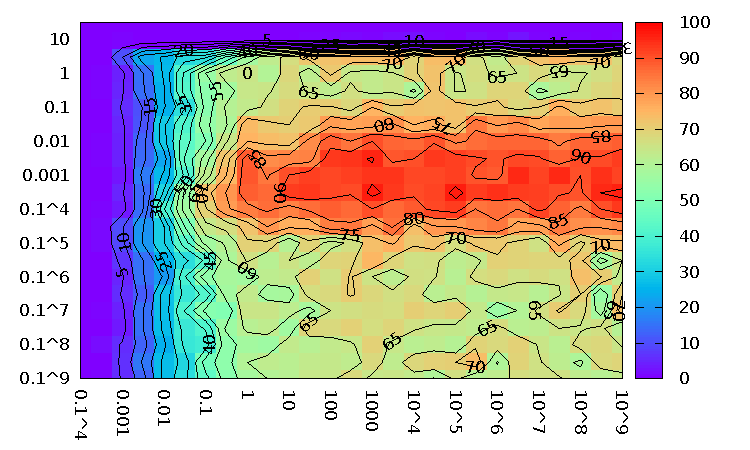
\includegraphics[width=0.48\textwidth]{img/tlr-auto4-success.pdf}   
  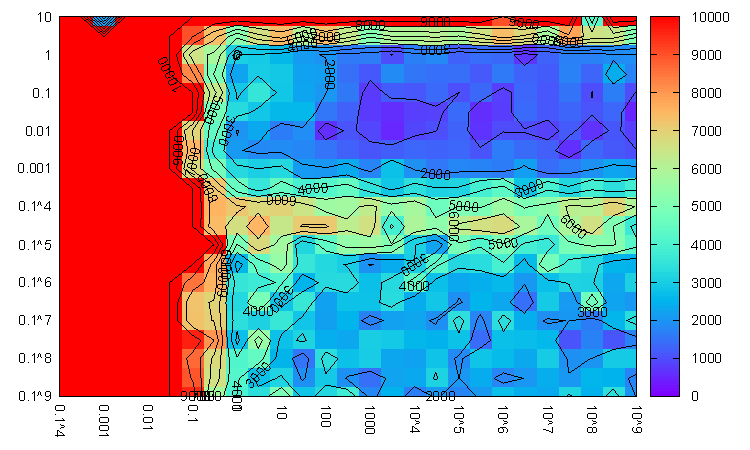
\includegraphics[width=0.48\textwidth]{img/tlr-auto4-epoch.pdf}     
  \caption{TLR success and epochs needed for successful networks on the \emph{4-2-4 encoder} task with $\sigma = 2.3$ and $\mu = 0.0$ best being $96.5\$$ with setting $\lambda_h=0.0003$ and $\lambda_v=1000.0$.}
  \label{fig:results-tlr-auto4-performance}
\end{figure}

Note the inconsistency between table~\ref{tab:results-cmp-auto4} where 93.12\% success was stated for TLR and in figure~\ref{fig:results-tlr-auto4-performance} it was 96.5\%. We can explain this by the \emph{law of big numbers}. In the first case we run 10,000 networks and therefore the result is likely to mirror the reality. In the second case only 200 networks were run for each$(\lambda_v,\,\lambda_h)$ pairs with having about 50 candidates for best achievers. Thus if we do little amount of runs for these 50 candidates it's likely that some them will achieve better than in reality. 

On the following figure~\ref{fig:results-tlr-auto4-epoch} we see that the success rate increases even after $10^5$ epochs and our intuition tells us that it will continue even after $10^6$ epoch. Also interesting is that $patSucc^B$ first follows $patSucc^F$ for about 100 epochs but then it stagnates at rate $\approx0.8$ and even it starts to drop a little. TODO explain, maybe an implementation error? It's so symmetric and weight update is independent on activation cimputation. 

%======== (2D) best TLR on ALL_SUCC x epoch (std-dev) ==========
\begin{figure}[H]
  \centering
  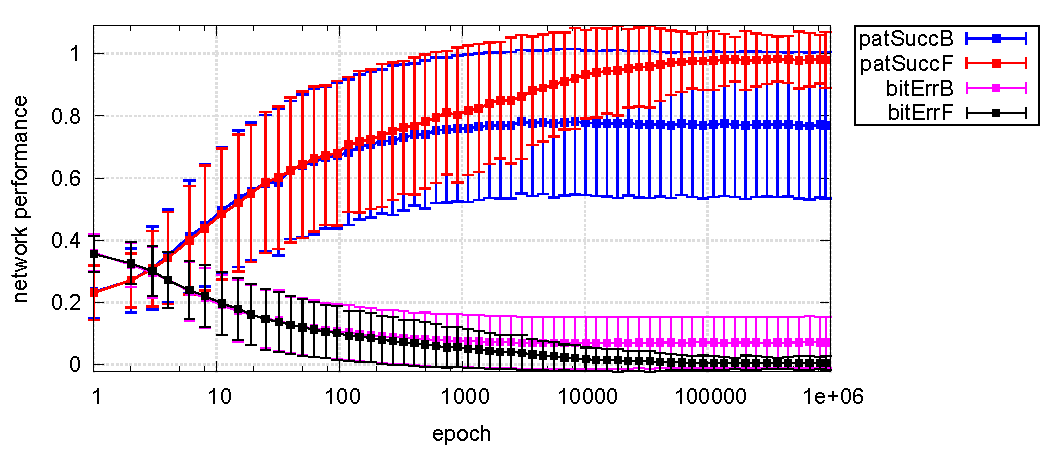
\includegraphics[width=0.48\textwidth]{img/tlr-auto4-best-perf.pdf}   
  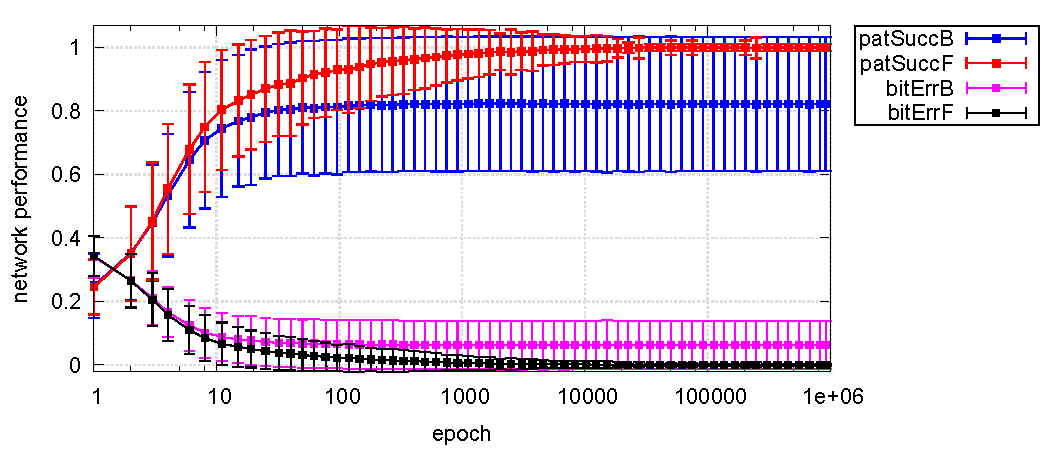
\includegraphics[width=0.48\textwidth]{img/tlr-auto4-best-can.pdf}      
  \caption{TLR success timeline for the \emph{4-2-4 encoder} task with $\lambda_h=0.0002$ and $\lambda_v=500$. Left without candidate selection and right with candidates selection.}
  \label{fig:results-tlr-auto4-epoch} 
\end{figure}

%============================================================
\subsubsection{Hidden activations}
\ref{sec:our-hidden-activation}  

On figures~\ref{fig:results-hidden-activations-bal} and~\ref{fig:results-hidden-activations-tlr} we show forward hidden activations. Each color represents the forward hidden representation of one of the four inputs in the \emph{4-2-4 encoder} task. As the hidden layer has size 2 it could be mapped to $(0,1)^2$. The activations started at the black dots and continued as outlined by the the lines. The numbers attached to the lines are the epoch numbers. 

The main difference between TLR and BAL seems to be the speed of activation change. In BAL on figure~\ref{fig:results-hidden-activations-bal} we have a step of size 0.6 which corresponds to four, one for each input, weight updates. And after some initial steps BAL tends to stop the activation change. This could be contributed to settling $|H^F-H^B| \approx \overrightarrow{0}$ as discussed in \ref{sec:our-hidden-activation}. 

Another source of error could be \emph{non--convex} hidden activation initializations. In the beginning the weight matrices are initialized by random what leads to random hidden activations. If they are also non--convex in the end then it's impossible to perfectly classify on the hidden--to--visible layer due the linear separability theorem discussed in section~\ref{sec:models-perceptron}. Thus the network must \emph{escape} the non--convex state which could introduce problems. 

%===== hidden activation timelines with commentaries (for TLR, BAL, GeneRec) 
% 2x success, 2x error (wrong settle, divergence) 

%TODO somehow divide so it will be visible together with explanation (left, right page 2x2, reduce...) 
%TODO should have also backward activations ... now we can only guess 
\begin{figure}[H]
  \centering
  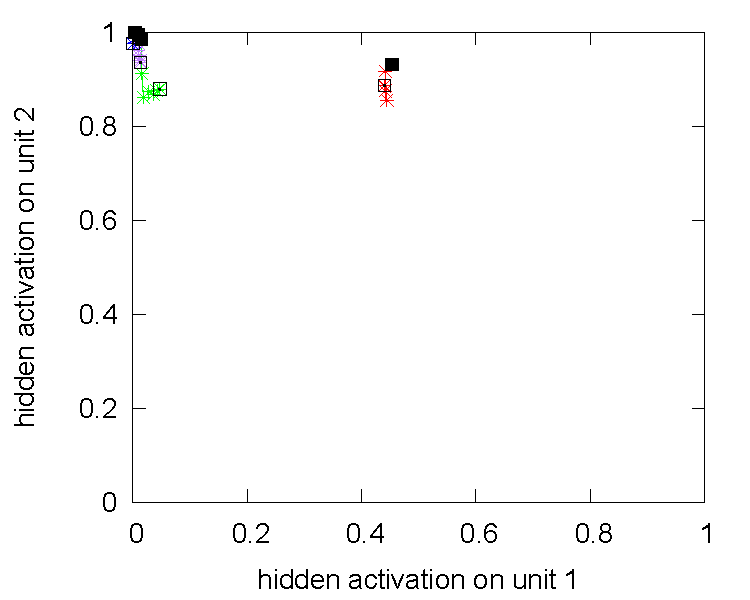
\includegraphics[width=0.48\textwidth]{img/hid-bal-bad-init.pdf}  
  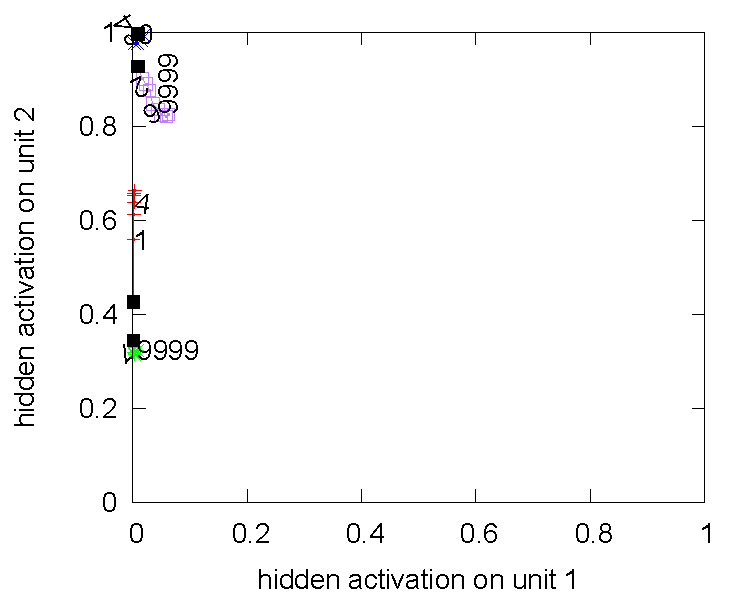
\includegraphics[width=0.48\textwidth]{img/hid-bal-bad-convex.pdf}  \\
  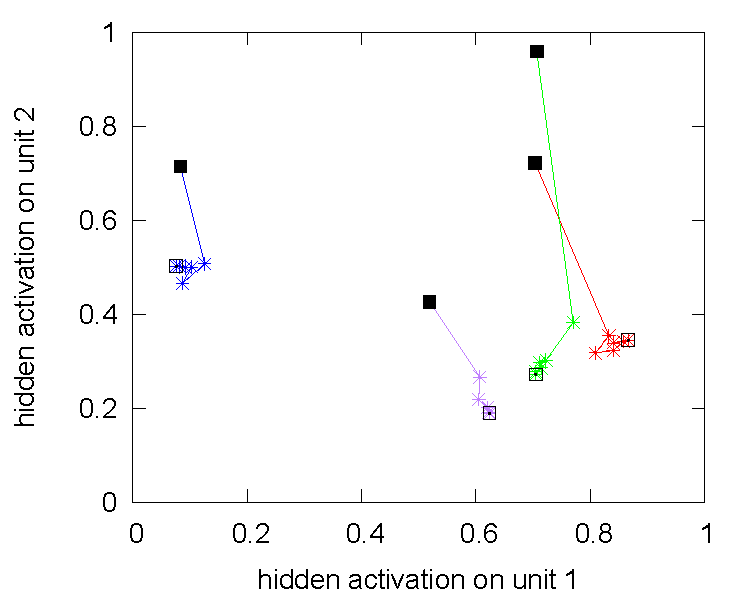
\includegraphics[width=0.48\textwidth]{img/hid-bal-bad-step.pdf}  
  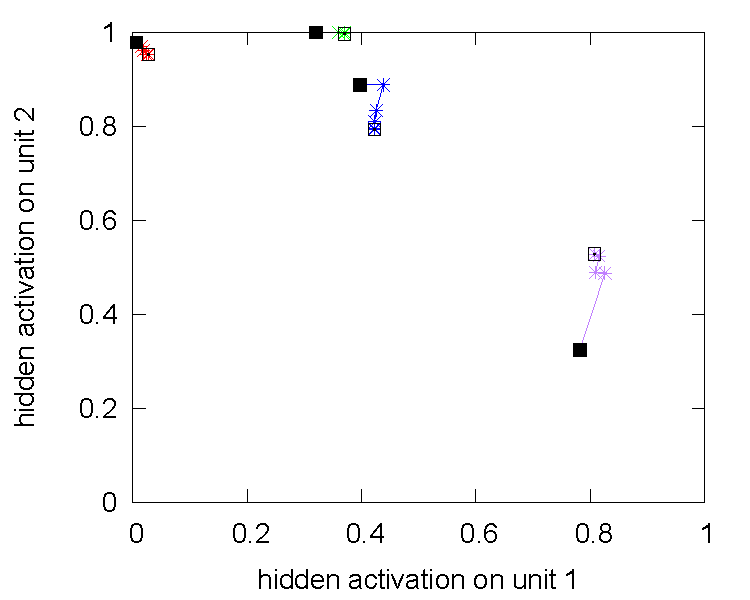
\includegraphics[width=0.48\textwidth]{img/hid-bal-bad-stagnation.pdf}  \\
  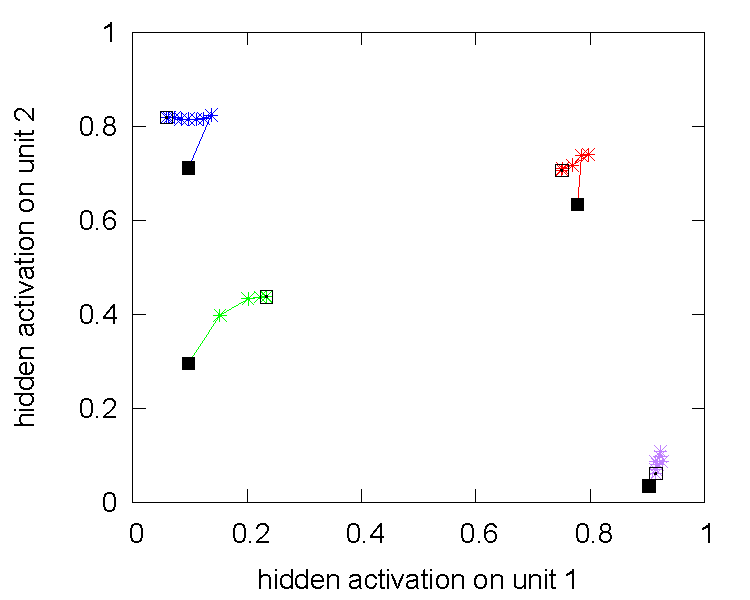
\includegraphics[width=0.48\textwidth]{img/hid-bal-good-init.pdf}  
  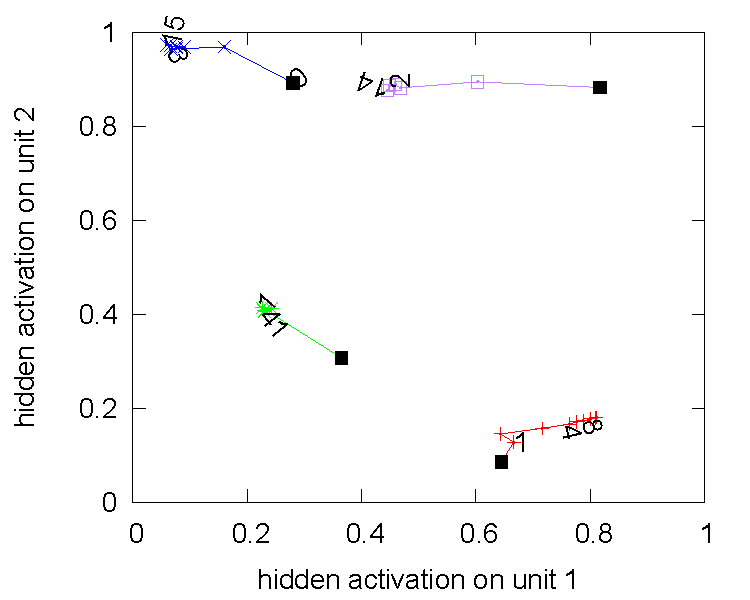
\includegraphics[width=0.48\textwidth]{img/hid-bal-good-convex.pdf}  \\
  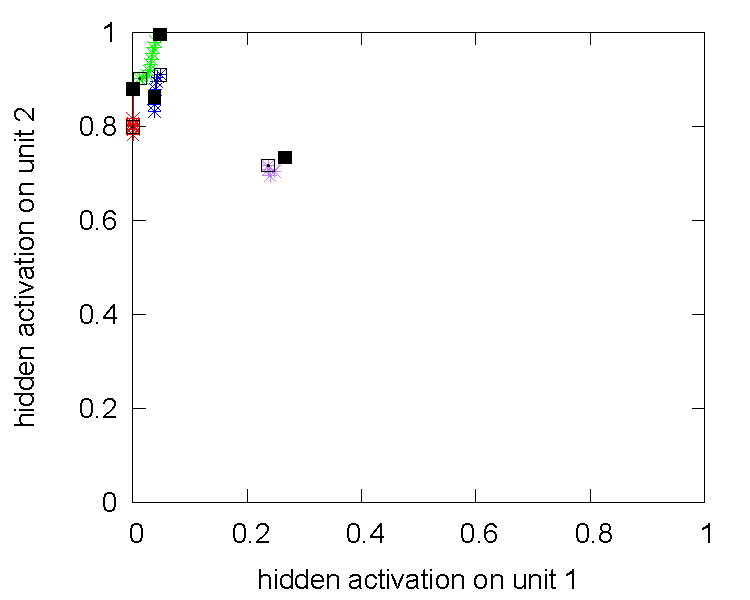
\includegraphics[width=0.48\textwidth]{img/hid-bal-good-step.pdf}  
  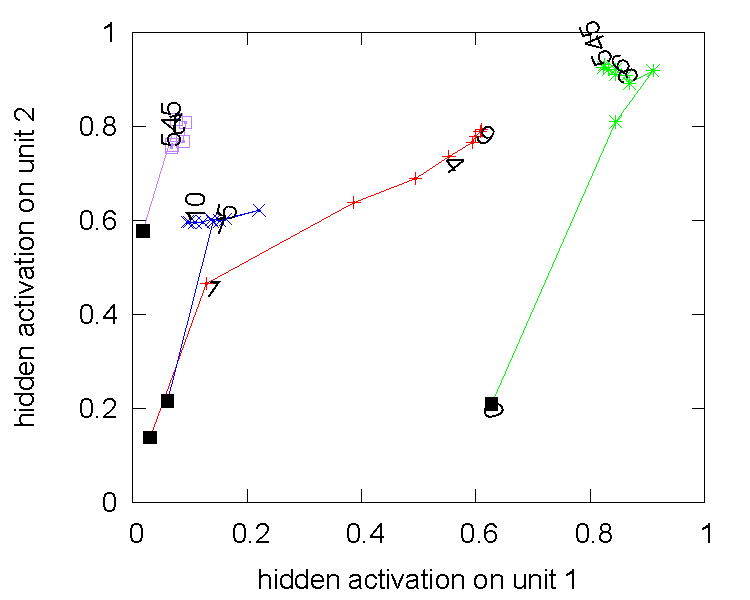
\includegraphics[width=0.48\textwidth]{img/hid-bal-good-stagnation.pdf}  \\ 
  \caption{\emph{BAL} hidden activations on the \emph{4-2-4 encoder}. Top $2\times2$ are {\bf un}successful networks and bottom $2\times2$ successful ones.}
  \label{fig:results-hidden-activations-bal}
\end{figure}

\begin{figure}[H]
  \centering
  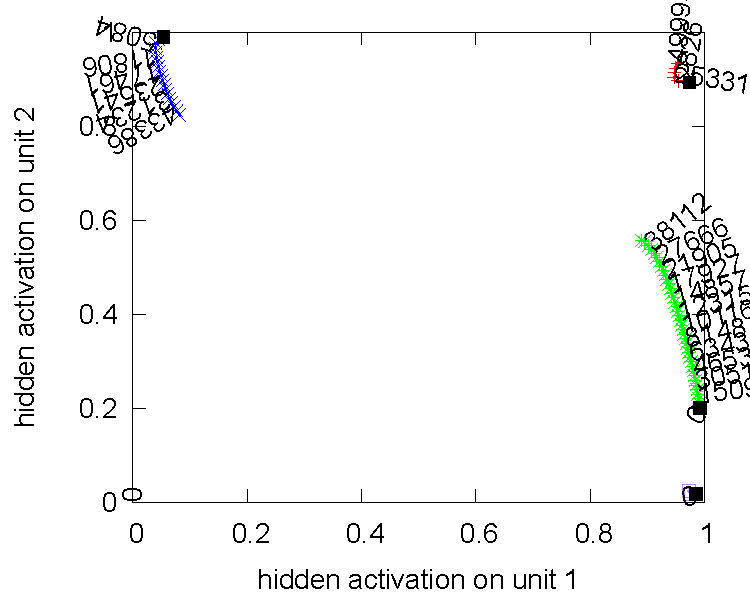
\includegraphics[width=0.48\textwidth]{img/hid-tlr-bad-static.pdf}  
  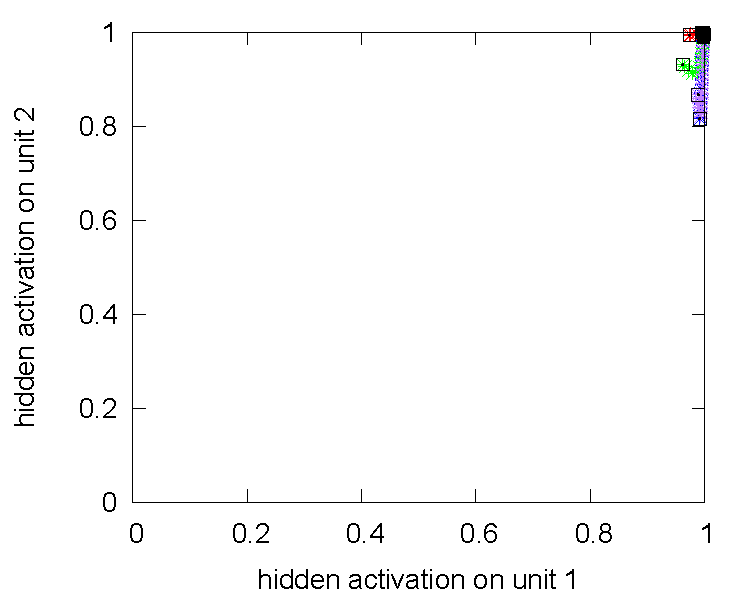
\includegraphics[width=0.48\textwidth]{img/hid-tlr-bad-tiny.pdf}  
  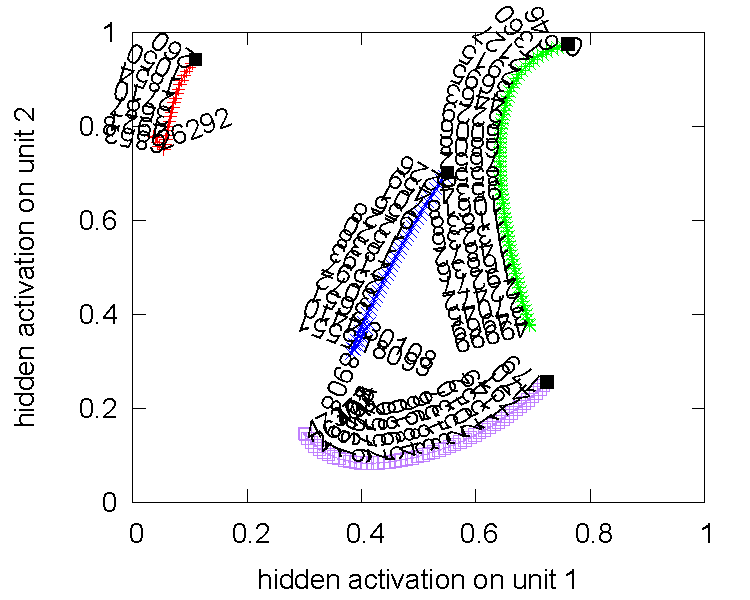
\includegraphics[width=0.48\textwidth]{img/hid-tlr-bad-init.pdf}  
  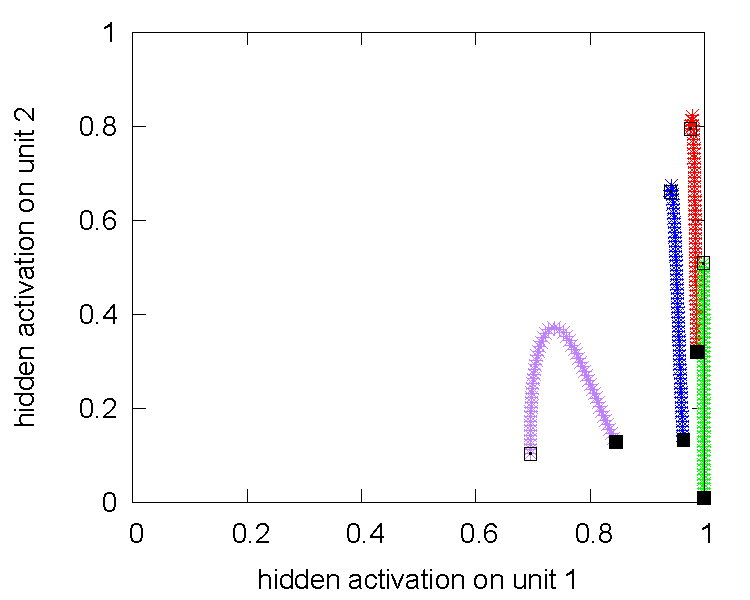
\includegraphics[width=0.48\textwidth]{img/hid-tlr-bad-weird.pdf}  
  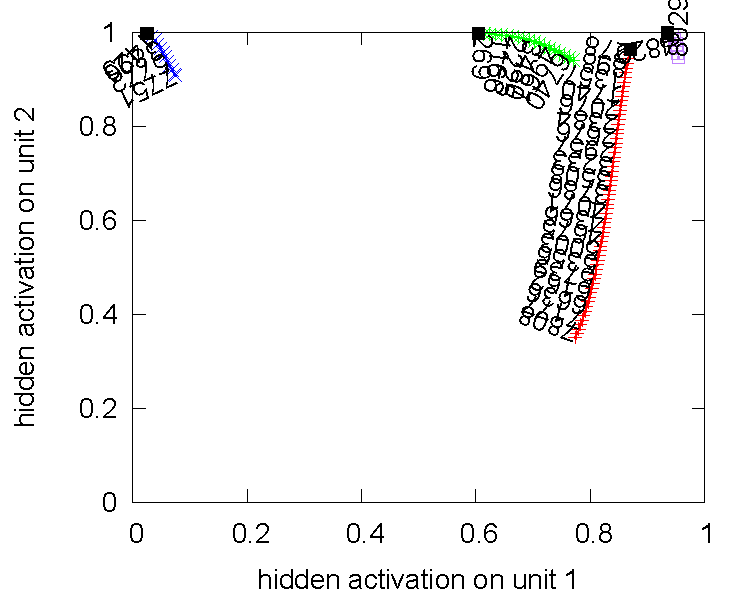
\includegraphics[width=0.48\textwidth]{img/hid-tlr-good-static.pdf}  
  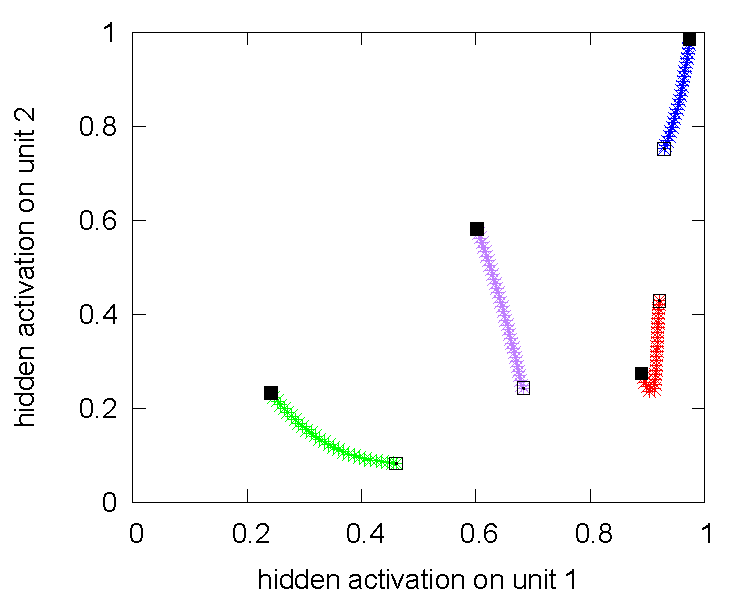
\includegraphics[width=0.48\textwidth]{img/hid-tlr-good-tiny.pdf}  
  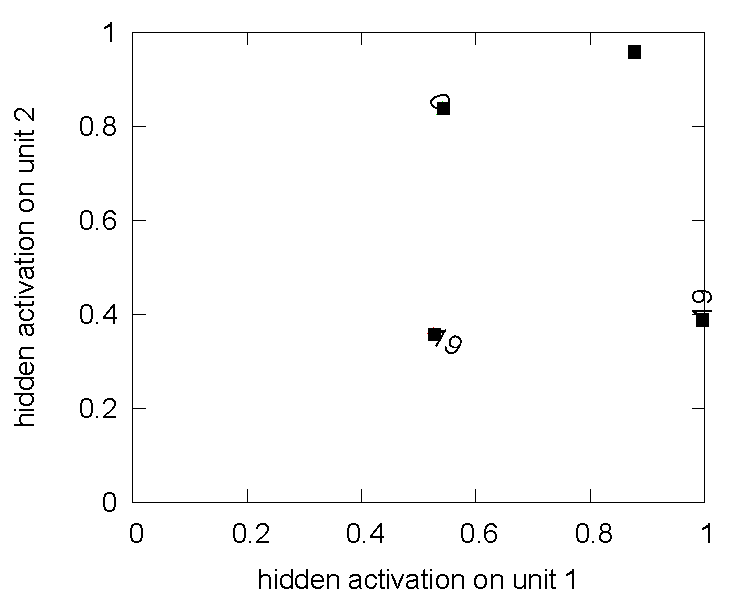
\includegraphics[width=0.48\textwidth]{img/hid-tlr-good-init.pdf}  
  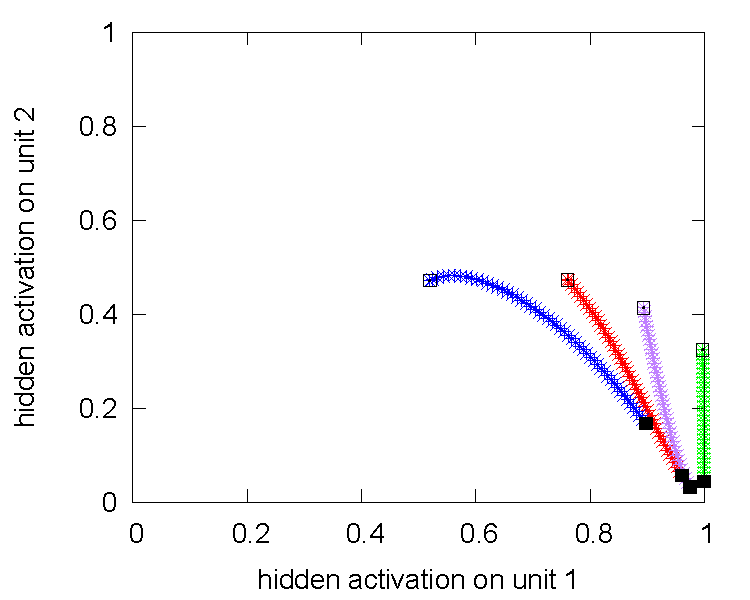
\includegraphics[width=0.48\textwidth]{img/hid-tlr-good-weird.pdf}  
  \caption{\emph{TLR} hidden activations on the \emph{4-2-4 encoder}. Top $2\times2$ are {\bf un}successful networks and bottom $2\times2$ successful ones.}
  \label{fig:results-hidden-activations-tlr}
\end{figure}

%============================================================
\subsubsection{Features}
\label{sec:results-auto4-bal-matrix-sim}

TODO[opt] feature to epoch of best (in worst we will throw away) 

\subsubsection{Other} 

\paragraph{Recirculation BAL.} 
%======== (3D) L1 x L2 x epochs =========
%======== (3D) L1 x L2 x patSuccF =========
\begin{figure}[H]
  \centering
  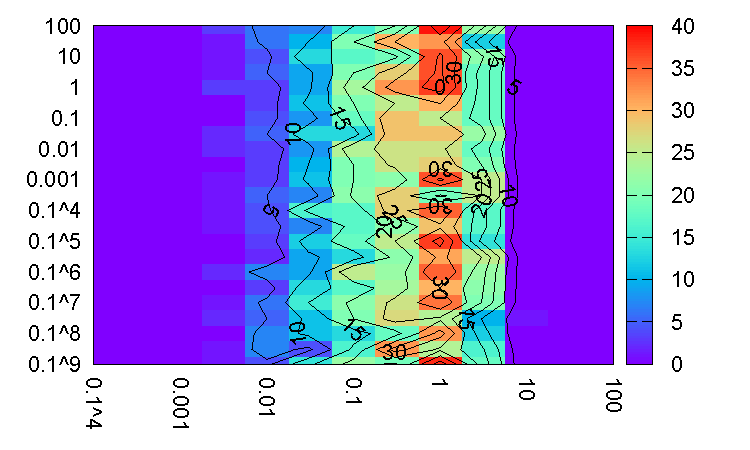
\includegraphics[width=0.48\textwidth]{img/bal-recirc-auto4-success.pdf}   
  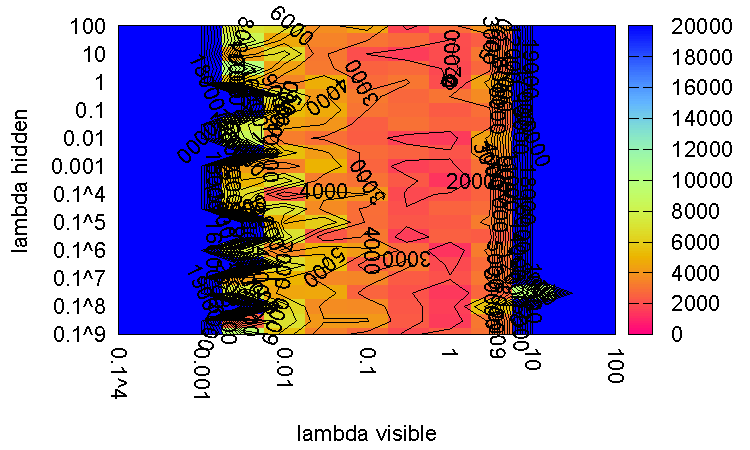
\includegraphics[width=0.48\textwidth]{img/bal-recirc-auto4-epoch.pdf}     
  \caption{BAL-recirc \ref{sec:our-bal-recirc} success and convergence on the \emph{4-2-4 Encoder} task with $\sigma = 2.3$ and $\mu = 0.0$.}
  \label{fig:results-bal-recirc-auto4-performance}
\end{figure}

\paragraph{Symmetric BAL.} 
\label{sec:our-bal-sym} 
\emph{Symmetric BAL (SymBAL)} is inspired by the necessary condition for convergence of GeneRec \citep{o1996bio} we set symmetric weights $W^{IH} = (W^{HI})^T$ and $W^{HO} = (W^{OH})^T$. We found no significant improvement when using this approach. TODO plot. 

\paragraph{GeneRec.} 
%======== (3D) L1 x L2 x epochs =========
%======== (3D) L1 x L2 x patSuccF =========
\begin{figure}[H]
  \centering
  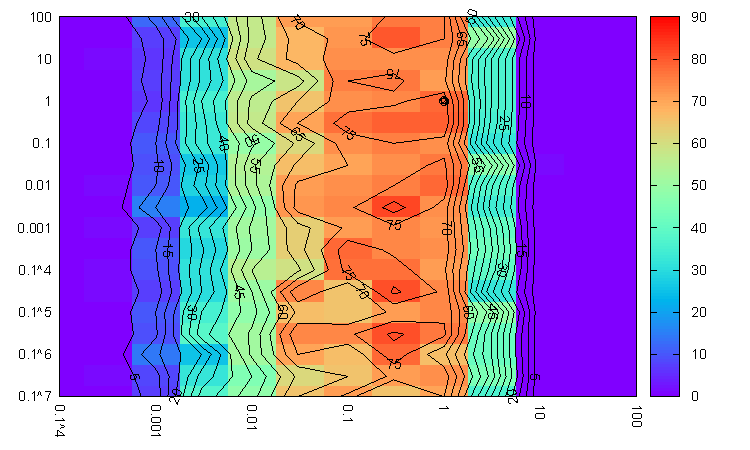
\includegraphics[width=0.48\textwidth]{img/generec-auto4-success.pdf}   
  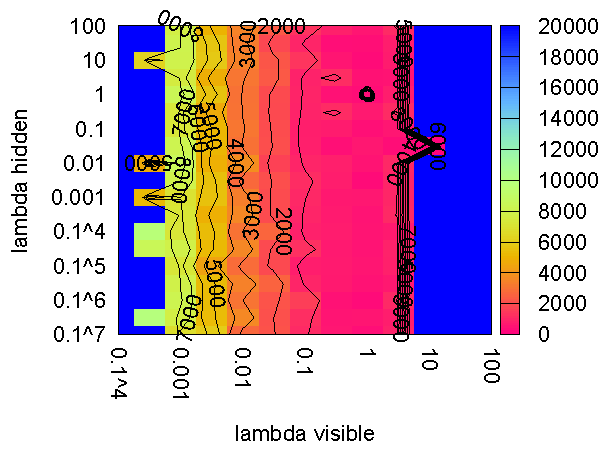
\includegraphics[width=0.48\textwidth]{img/generec-auto4-epoch.pdf}     
  \caption{GeneRec \ref{sec:models-generec} success and convergence on the \emph{4-2-4 Encoder} task with $\sigma = 2.3$ and $\mu = 0.0$.}
  \label{fig:results-generec-auto4-performance}
\end{figure}


\subsubsection{Conclusion} 
\label{sec:tlr-auto4-conclusion} 

TODO Explain / Make up hypotheses why it behaves as measured (Future work). \\
